\documentclass[10pt,a4paper]{article}
\usepackage[latin1]{inputenc}
\usepackage[english]{babel}
\usepackage{amsmath}
\usepackage{amsfonts}
\usepackage{amssymb}
\usepackage{graphicx}
\usepackage{fancyhdr}
\usepackage{lastpage}
\usepackage{multirow}

%Include and define  c code
\usepackage{listings}
\usepackage{color}
\usepackage{textcomp}
\definecolor{listinggray}{gray}{0.9}
\definecolor{lbcolor}{rgb}{0.9,0.9,0.9}
\lstset{
	language=C,
	keywordstyle=\bfseries\ttfamily\color[rgb]{0,0,1},
	identifierstyle=\ttfamily,
	commentstyle=\color[rgb]{0.133,0.545,0.133},
	stringstyle=\ttfamily\color[rgb]{0.627,0.126,0.941},
	showstringspaces=false,
	basicstyle=\small,
	numberstyle=\footnotesize,
	numbers=left,
	stepnumber=1,
	numbersep=10pt,
	tabsize=2,
	breaklines=true,
	prebreak = \raisebox{0ex}[0ex][0ex]{\ensuremath{\hookleftarrow}},
	breakatwhitespace=false,
	aboveskip={1.5\baselineskip},
  columns=fixed,
  upquote=true,
  extendedchars=true,
 frame=single,
 backgroundcolor=\color{lbcolor},
}

\oddsidemargin  -0.5cm
\evensidemargin 0.0cm
\textwidth      17.25cm
\headheight     1.0cm
\headsep		0.7cm
\topmargin      -0.5cm
\textheight		22.0cm

\pagestyle{fancy}
\lhead{Exercise 5}
\chead{EEMB1}
\rhead{\thepage\ of \pageref{LastPage}}
\lfoot{Theis Christensen\\Paulo Fontes\\Dennis Madsen}
\cfoot{Team3}
\rfoot{\today}
\renewcommand{\headrulewidth}{0.4pt}
\renewcommand{\footrulewidth}{0.4pt}
\begin{document}
\part*{EMB 2010 Team3 Exercise5}
\section{Introduction}
In this exercise we  are able to create a 2 channel voltmeter that displays the measured voltage on the LCD display using SWIM ( Simple Window Interface Manager).
A driver will be created for the LPC 2478 built-in analog to digital converter (adc).
A draw file is created to make easy the development of a graphical layout on the LCD display, making possible further improvements. 
\\ \newline
In the below figure is seen how the clock is routed through the system to the ADC block. The clock value putted into the block is 28.8MHz.
\\ \newline
\begin{figure}[h!]
   \centering
   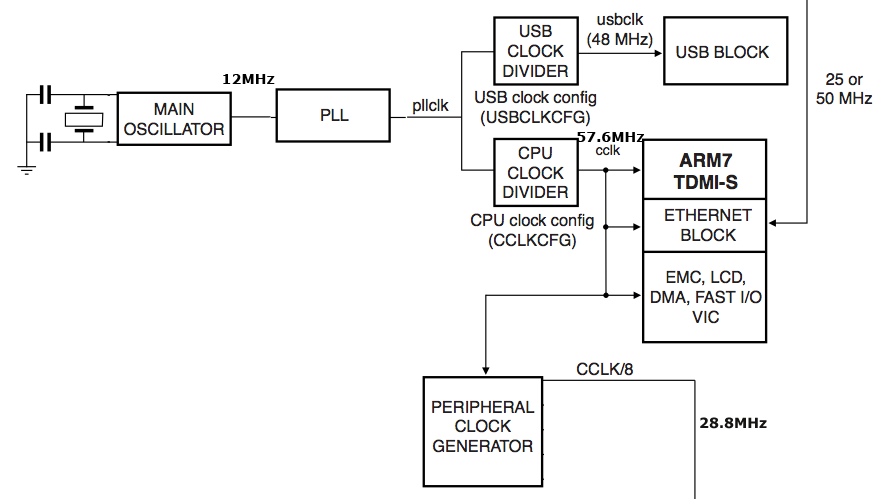
\includegraphics[width=1\textwidth]{peripheral_clock_gen.png}
   \caption{Peripheral clock scaling}
   \label{fig:example}
\end{figure}

\newpage
\section{Initialization}

The ADC is initialised by the function initAdc(unsigned char CLKDIV, unsigned char CLKS, unsigned short SEL).
\\ \newline
The initialisation starts by powering up (enabling) the ADC register this is disabled at the reset for power saving purpose since it may consume power that is not clock dependent.
\begin{lstlisting} 
	PCONP |= (1<<12);
 \end{lstlisting}

The clock has to be set and scaled since the ADC works at a lower frequency this is done by setting the peripheral clock selection to PCLK\_ADC (bit 25 and 24), this will control the clock rate to be suitable for the analog to digital conversion.
\begin{lstlisting} 
	PCLKSEL0 |= ((1<<25) | (1<<24));
 \end{lstlisting}


Pins are selected using a switch case, so we initialise the defined ADC that was send by parameter as SEL. Some of this pins have more than one physical connections, they can be connected to other component on the embedded artists board, as example pin AD0.0, AD0.1, AD0.2 are connected to the accelerometer, so the jumpers have to be changed is the accelerometer measure is not needed. In this example AD0.2 is using the red potentiometer over the display.

\begin{lstlisting}
switch (SEL){
		case 0: PINSEL1 |= (1<<14); break; // Selects p0.23
		case 1: PINSEL1 |= (1<<16); break; // Selects p0.24
		case 2: PINSEL1 |= (1<<18); break; // Selects p0.25
		case 3: PINSEL1 |= (1<<20); break; // Selects p0.26
		case 4: PINSEL3 |= (1<<28) | (1<<29); break; // Selects p1.30
		case 5: PINSEL3 |= (1<<30) | (1<<31); break; // Selects p1.31
		case 6: PINSEL0 |= (1<<24) | (1<<25); break; // Selects p0.12
		case 7: PINSEL0 |= (1<<26) | (1<<27); break; // Selects p0.13
		default: break;
	}
\end{lstlisting}


A\/D control register makes it possible to setup which channel to convert, timing, modes and start trigger if needed. \\
The clock is set by CLKDIV ( clock division bit 8 ), this value plus one is divided by the PCLK defined before, this should be less or equal to 4.5MHz. \\
CLKS ( bit 17 ) define the number of clock to be use in each conversion, this can be translate as as accuracy, number of bits from 10 to 3 bits conversion.
The a/d converter is set as operational setting PDN (bit 21) to high.

\begin{lstlisting}
AD0CR = ((CLKDIV<<8) | (CLKS<<17) | (1<<21));
\end{lstlisting}

\newpage

\section{Getting Values}
Reading data from the ADC register is performed on function getAdc, this will be explained above.

\begin{lstlisting}
	// SEL:  ADC pin 
	unsigned int getAdc(unsigned short SEL)
\end{lstlisting}

When starting a new conversion we need to be sure that the register is free since we can only make a conversion from one A/D channel at time. \\ A pin is select and the conversion starts, when the conversion is finish a flag will rise at the correspondent A/D channel (AD0DR0:7), the value will be assigned to the variable unsigned int aVal, a timeout will ensure that the program is not going to stuck waiting for the done signal (bit 31).\\ When the conversion is done the the value is shift so it fits a value from 0 to 1023.

\begin{lstlisting}
// Reset AOCR Register since only one of these bits should be 1.
	AD0CR &= 0xFFFFFF00;

	//Start reading on ADC SEL.
	AD0CR |= (1<<24) | (1<<SEL);

   /*	Wait for the selected channel to finish converting
	*	If it takes to long the function returns 0 (Timeout)
	*/
	switch(SEL){
	case 0:
		while((AD0DR0 & (1<<31)) == 0 && (timeout < 10000)) timeout++;
		aVal = (AD0DR0 & 0x0000FFC0);
		break;
	case 1:
		while((AD0DR1 & (1<<31)) == 0 && (timeout < 10000)) timeout++;
		aVal = (AD0DR1 & 0x0000FFC0);
		break;
	(...)
	case 6:
		while((AD0DR6 & (1<<31)) == 0 && (timeout < 10000)) timeout++;
		aVal = (AD0DR6 & 0x0000FFC0);
		break;
	case 7:
		while((AD0DR7 & (1<<31)) == 0 && (timeout < 10000)) timeout++;
		aVal = (AD0DR7 & 0x0000FFC0);
		break;
	default:
		return 0;
		break;
	}

	// Stop ADC reading avoid glitch on readings.
	AD0CR &= 0xF8FFFFFF;

	//The value is shift 6 to fit the value 0-1023 (10 bit value)
	return (aVal >> 6);
\end{lstlisting}

\newpage

\section{SWIM - Simple Window Interface Management}

SWIM is a basic graphical library develop for NXP LPC products. This library allows developers to quickly implement a system with basic graphical windows. \\ Enabling the possibility of easily draw bail graphics primitives such as lines squares and text.

To make the code more readable a new file was created draw.c, this file has already code to draw objects such as horizontal / vertical bars, makes easy to write to a certain position of the screen.

With this file we were able of quickly create different ADC windows.

draw is documented with help of doxygen in appendix.

The program exer\_app.c will be use as example.
The SPI communication is initialised so we can send data to the LCD display.

\begin{lstlisting}
	/* SSD1289 fclk max 13MHz, clk HI idle, MSB first
	 * SPIInit(wClock, nFramesize, bCPHA, bCPOL, bLSBF)
	 */
	SPIInit(CLK5M, 8, 0, 1, 0);

	/* open and init LCD */
	open_lcd();

	// Define Color scheme
	COLOR_T *fblog;

	// Set LCD frame buffer address
	fblog = (COLOR_T *) EA2478_LCD_FRAME_BUF;
}

\end{lstlisting}

With the SPI communication set, we can start using SWIM to make the static layout and configurations, this is going to be all the graphics that don't change during the running program such as title and signature and setting the font size.

\begin{lstlisting}

	// Create a SWIM window
	swim_window_open(&win1, LCD_DISPLAY.pixels_per_line, LCD_DISPLAY.lines_per_panel, fblog, 0, 0,
			(LCD_DISPLAY.pixels_per_line - 1), (LCD_DISPLAY.lines_per_panel - 1), 1, LIGHTGRAY, WHITE, LIGHTGRAY);

	// select the font to use
	swim_set_font(&win1, (FONT_T *) &FONT);

	// set the pen color to use
	swim_set_pen_color(&win1, WHITE);

	// Add a title bar
	swim_set_title(&win1, " ADC 1 & 2", BLACK);

	//select the font to use
	swim_set_font(&win1, (FONT_T *) &font_rom8x16);

	// Writes Team 3 Signature
	signature(&win1);

}

\end{lstlisting}
 
All the dynamic graphics that are constantly changed are inside a while loop, where the AD channel is read and converted to a graphical representation as a vertical bar.

\begin{lstlisting}
	// 2 vertical bars draw on the window screen.
	vBar(&win1,60, 80, 50, 140, (getAdc(1)*330/1023), "V","ADC1", BLUE, 330);
	vBar(&win1,120, 80, 50, 140, (getAdc(2)*330/1023), "V","ADC2", BLUE, 330);
	
\end{lstlisting}


\begin{lstlisting}
Our main function:

int main(void){

	// SETS UP BASIC PLATFORM
	lowLevelInit(); 		
	
	// SETS UP THE SDRAM (The framebuffer)
	SDRAMInit(); 

	// Initialize ADC window
	init_lcd_exer();

	while(1){
		// Updates ADC graphics.
		update_lcd_exer();
	}

	return 0;
}
\end{lstlisting}


\section{It's alive...}



\begin{tabular}{ p{8cm}  p{8cm} }
  Exercise 5 & Accelerometer  \\
   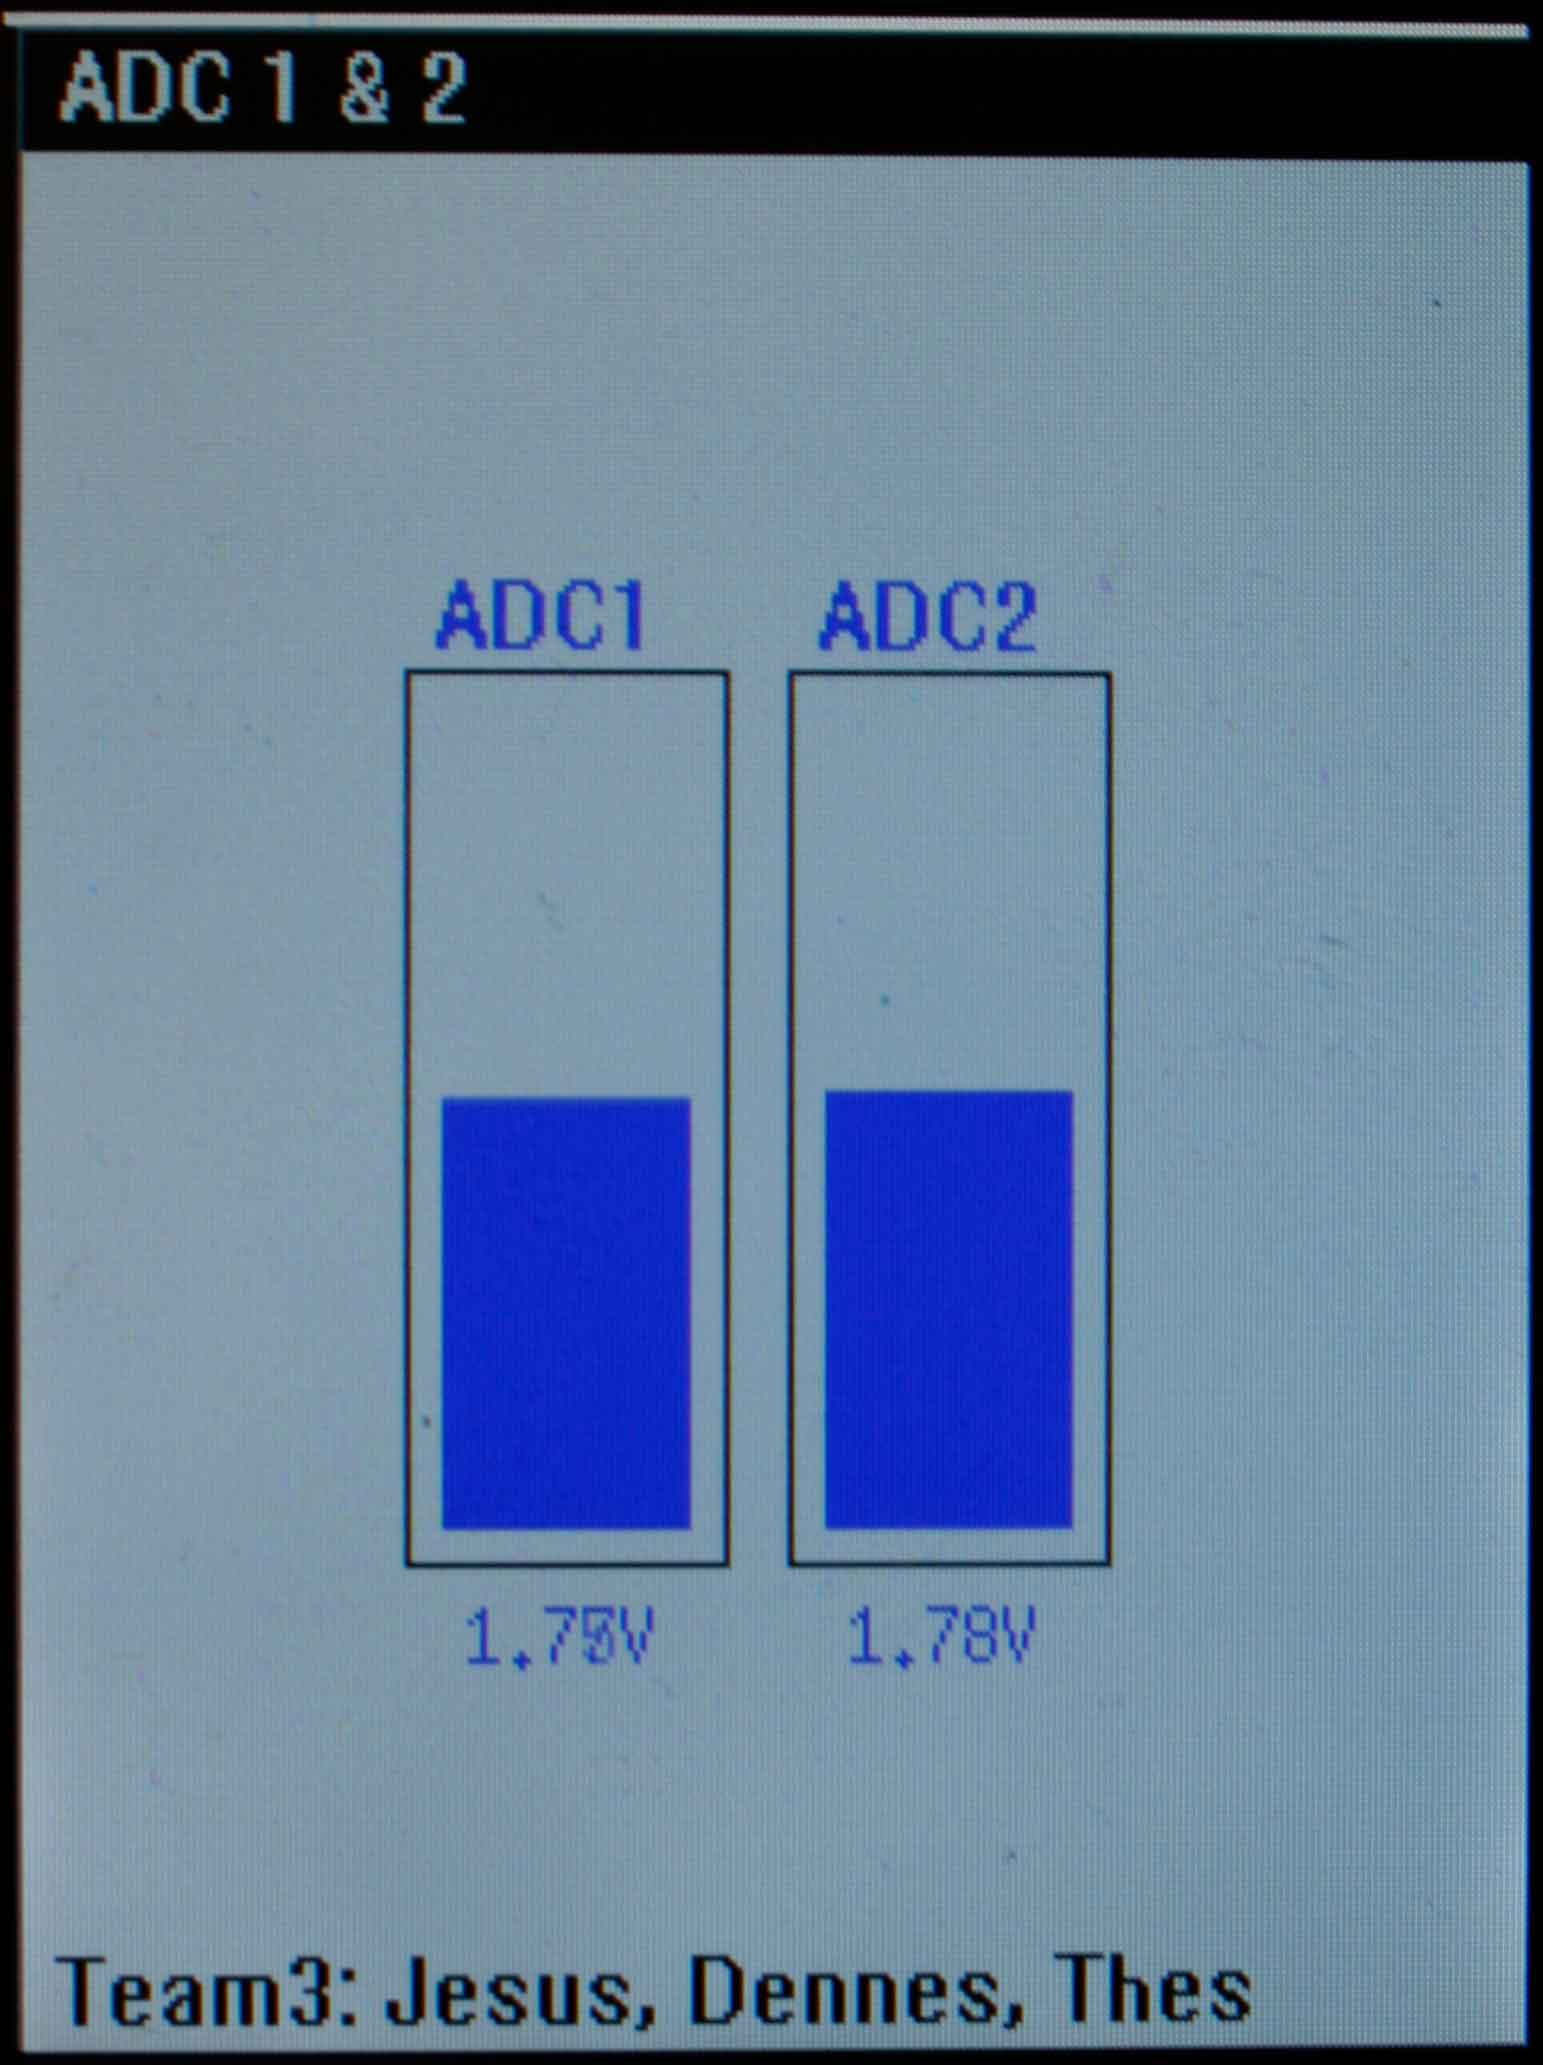
\includegraphics[width=0.4\textwidth]{adc12.jpg} & 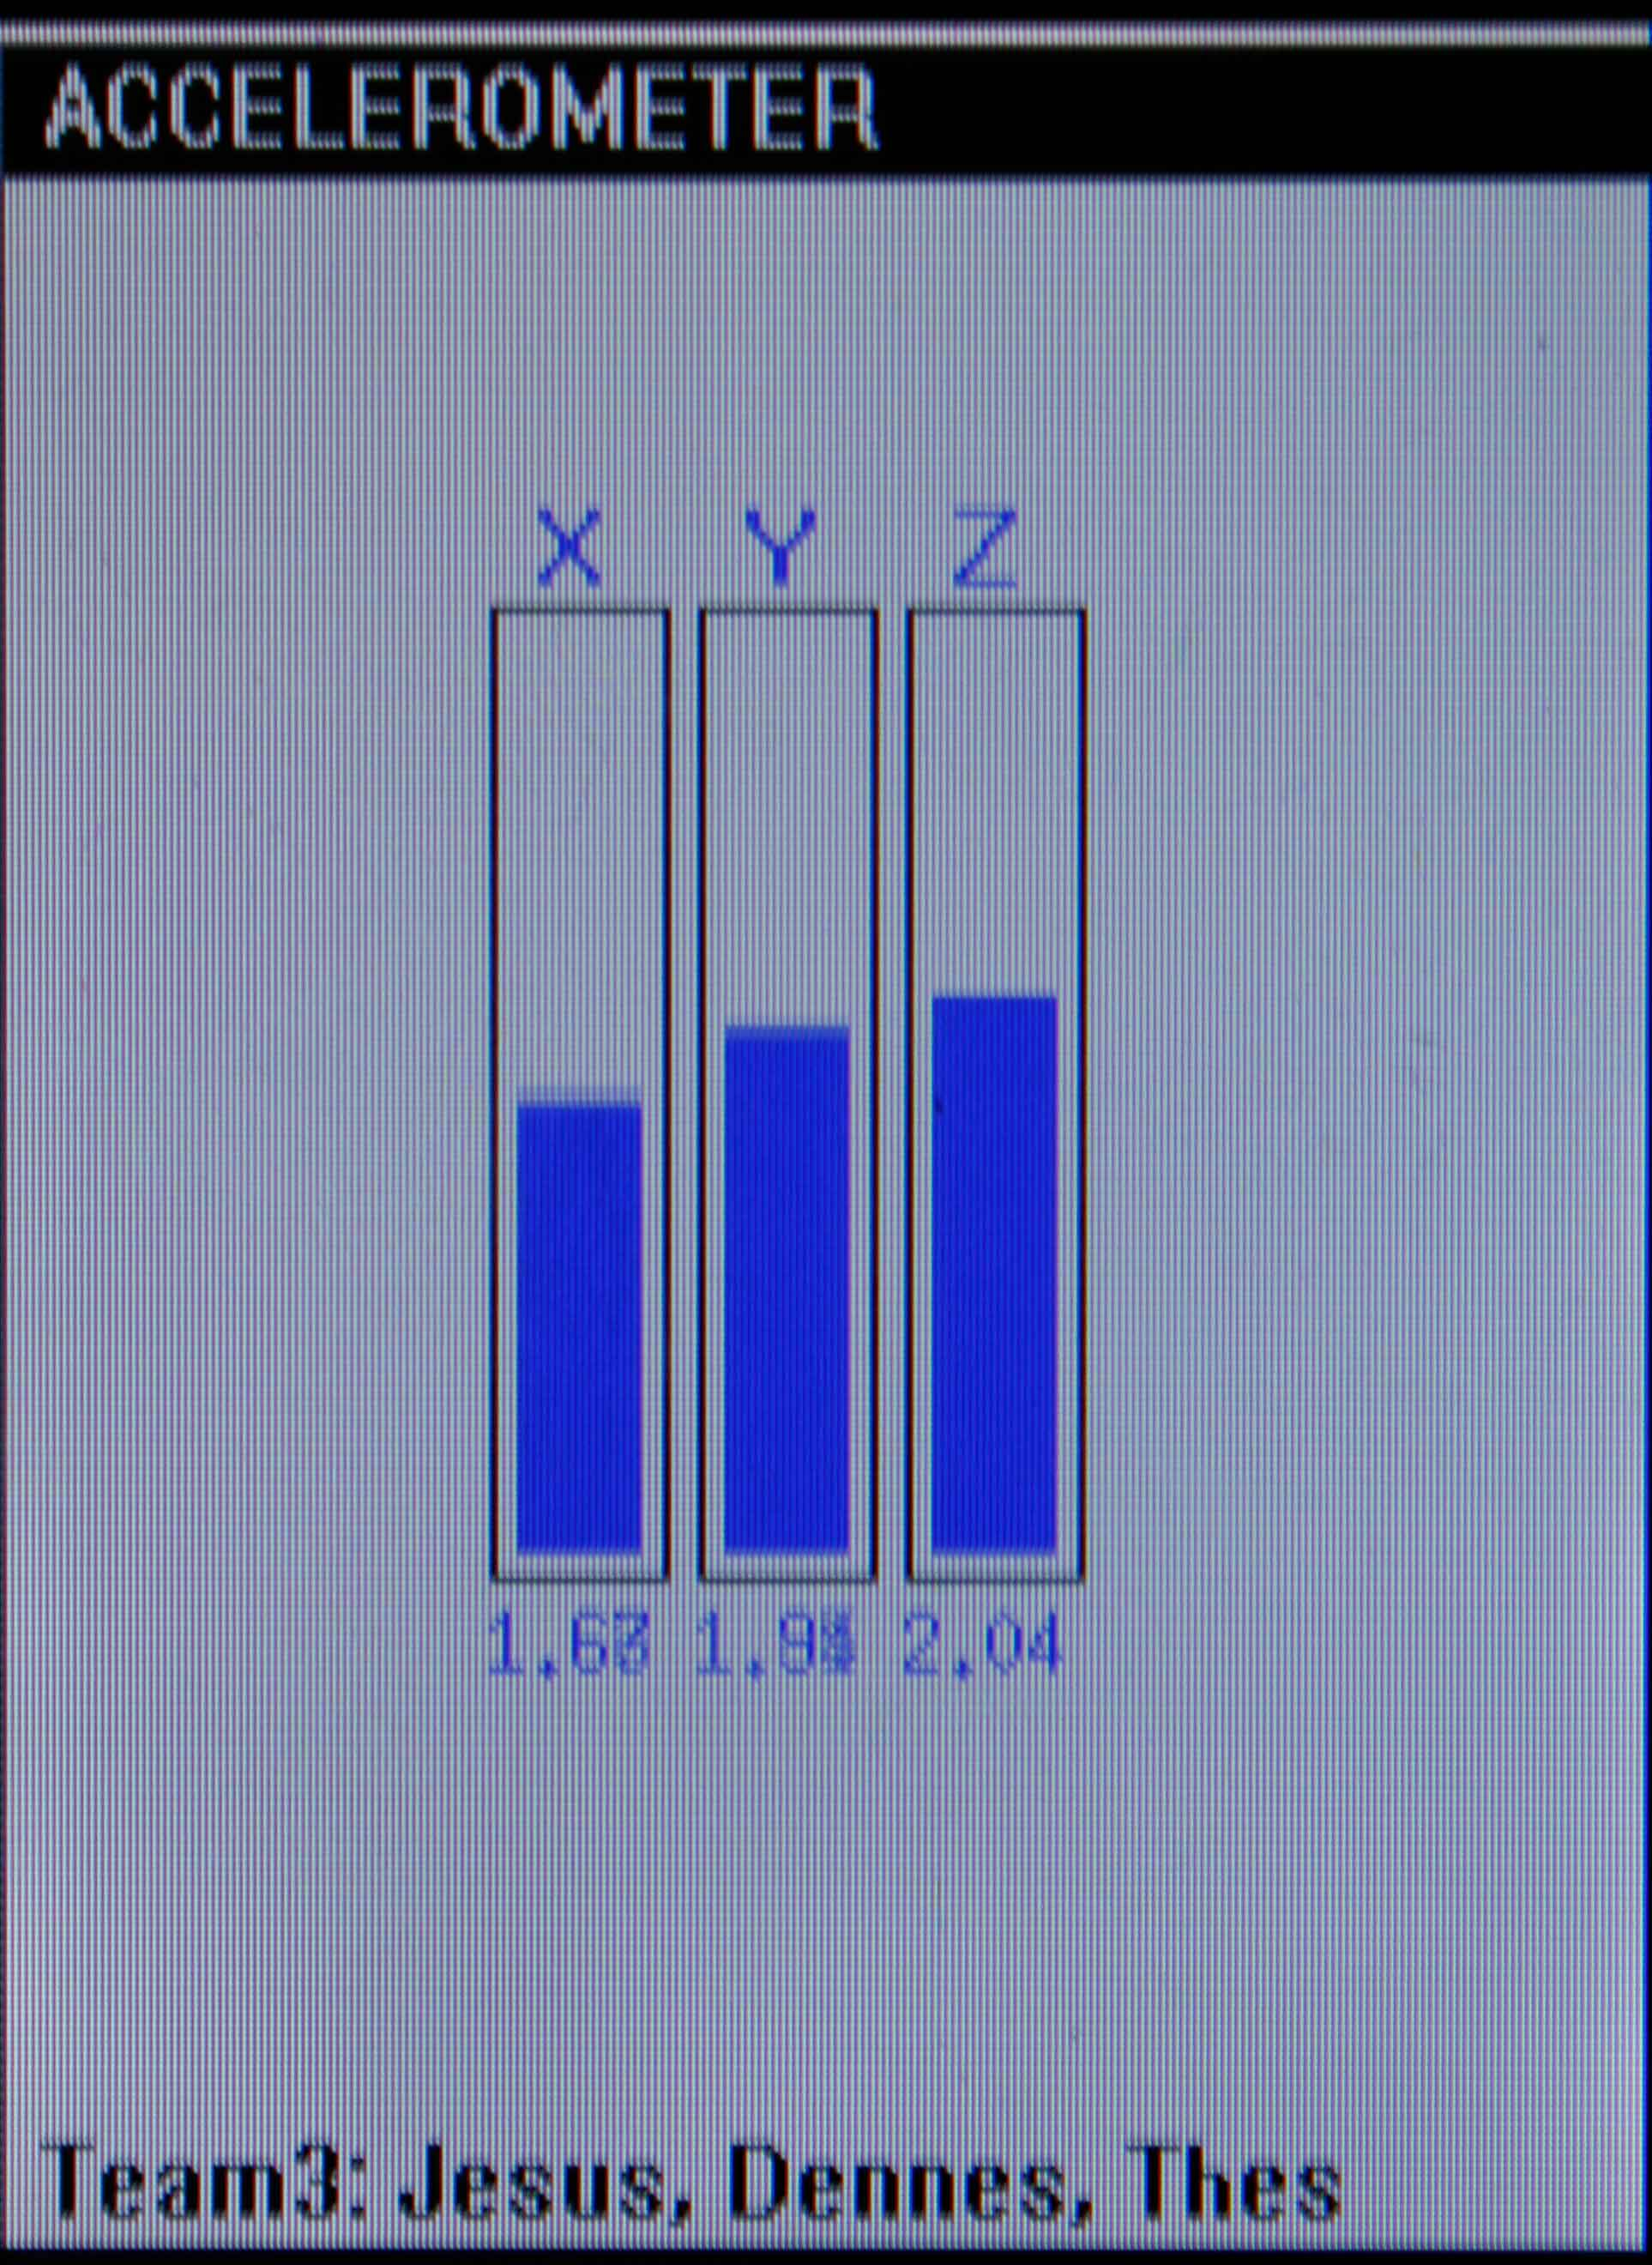
\includegraphics[width=0.39\textwidth]{accel.jpg}  \\
  exer\_app.c : Perform the requirements of the exercise & accel\_app.c : Use the accelerometer ( A7260 ) to get the analog value from X, Y and Z. \\
  ~ &~ \\
  ADC's & Potentiometer\\
  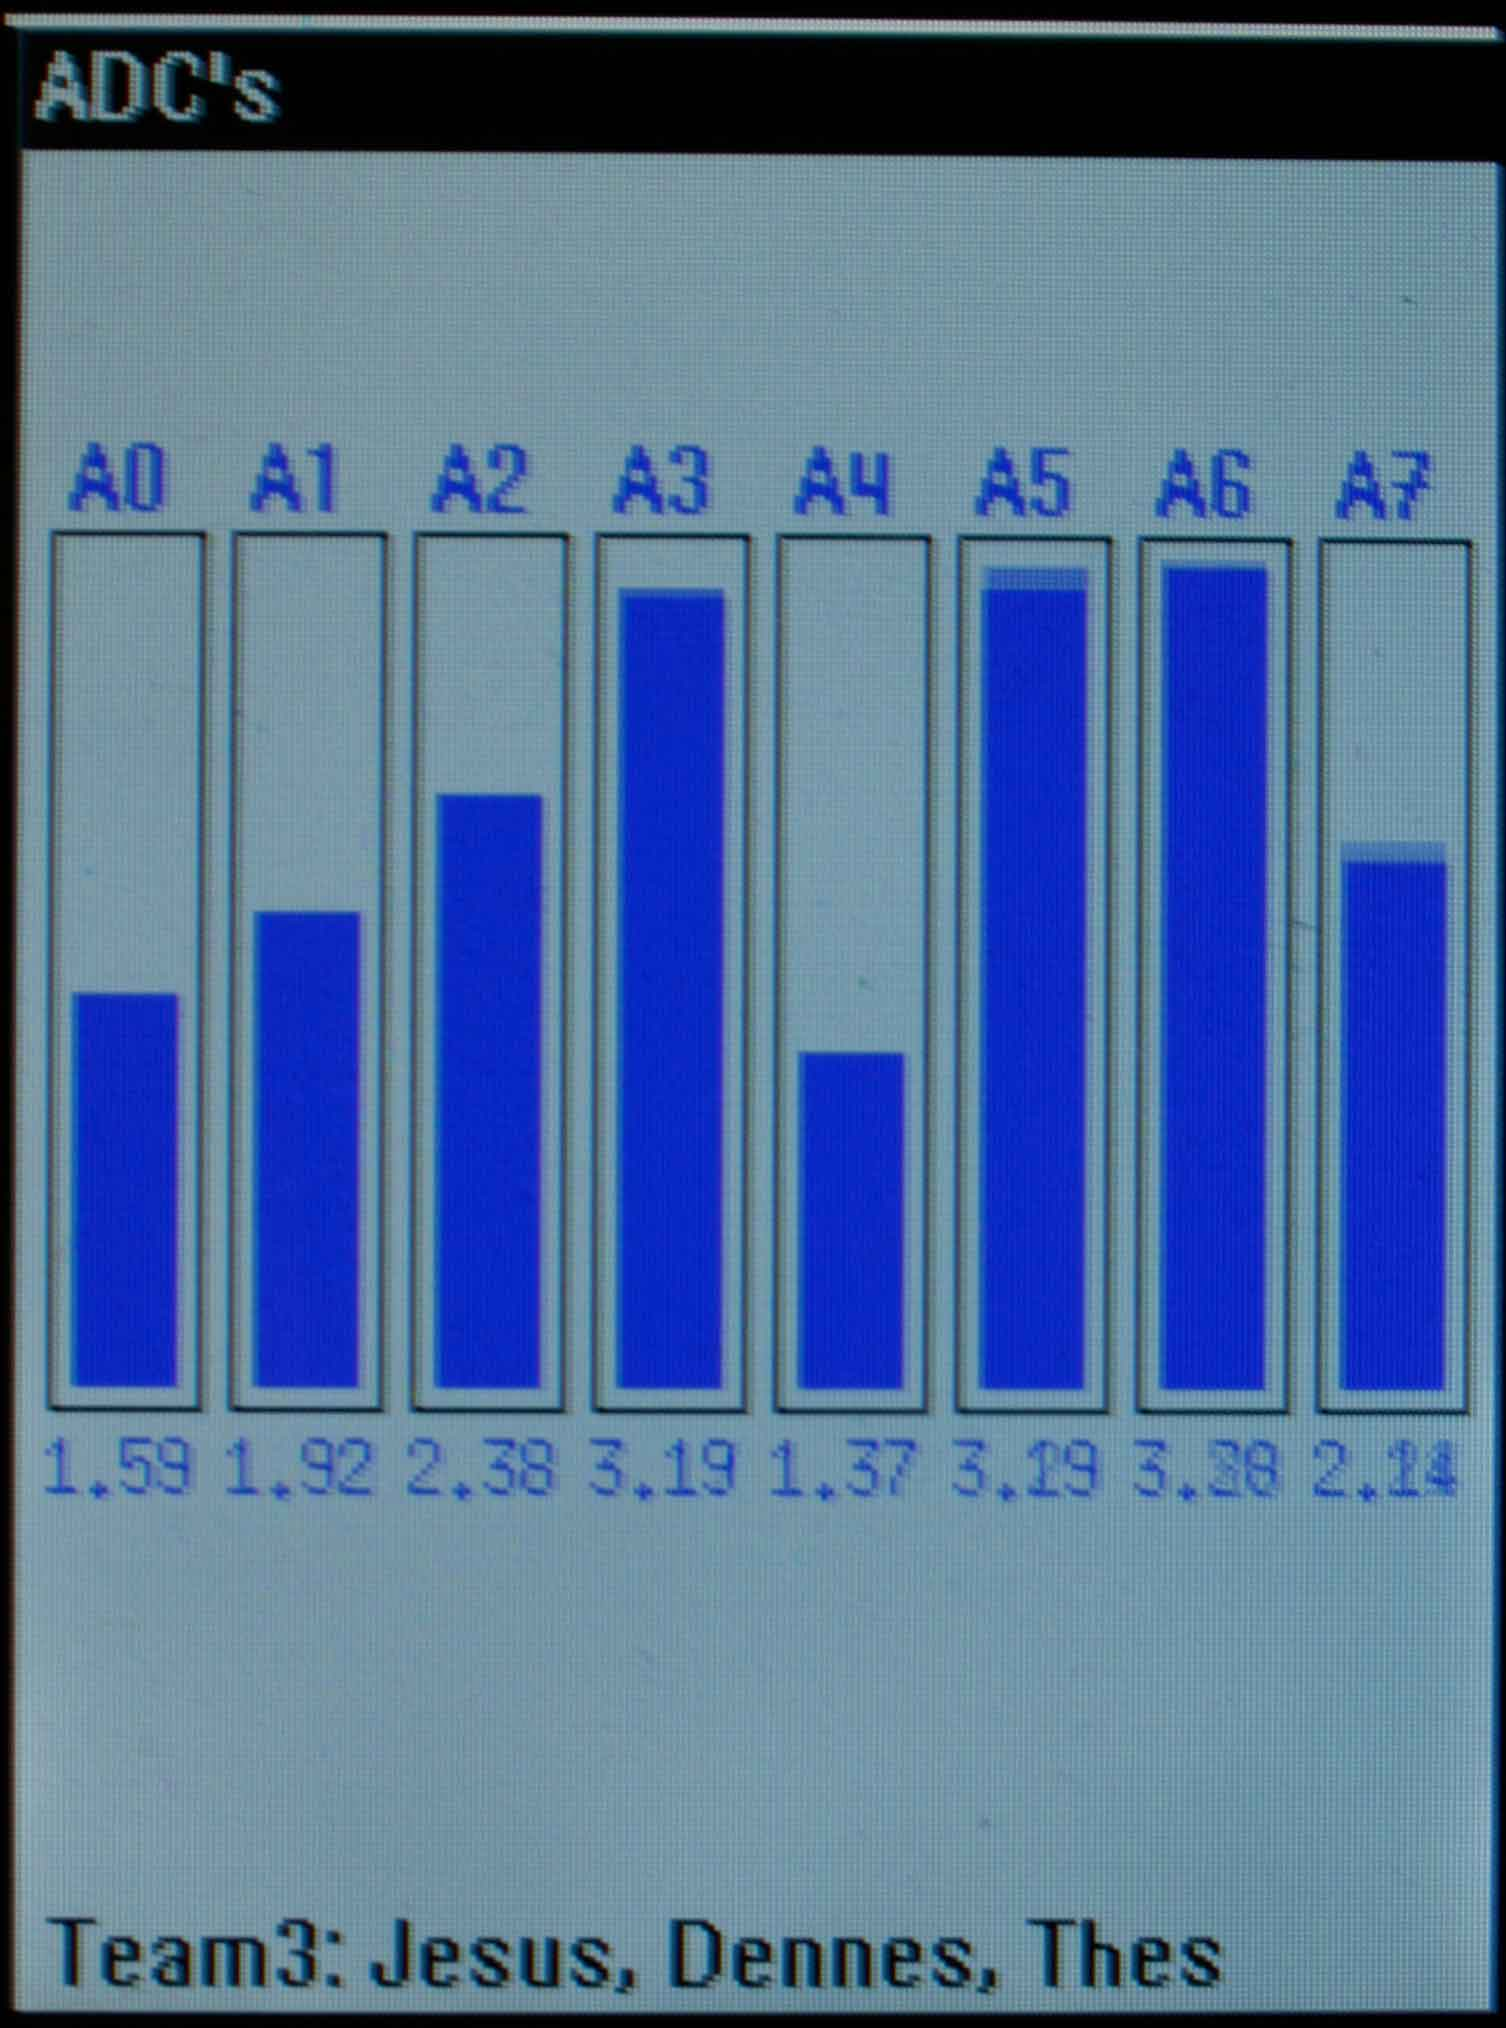
\includegraphics[width=0.4\textwidth]{adcs.jpg} & 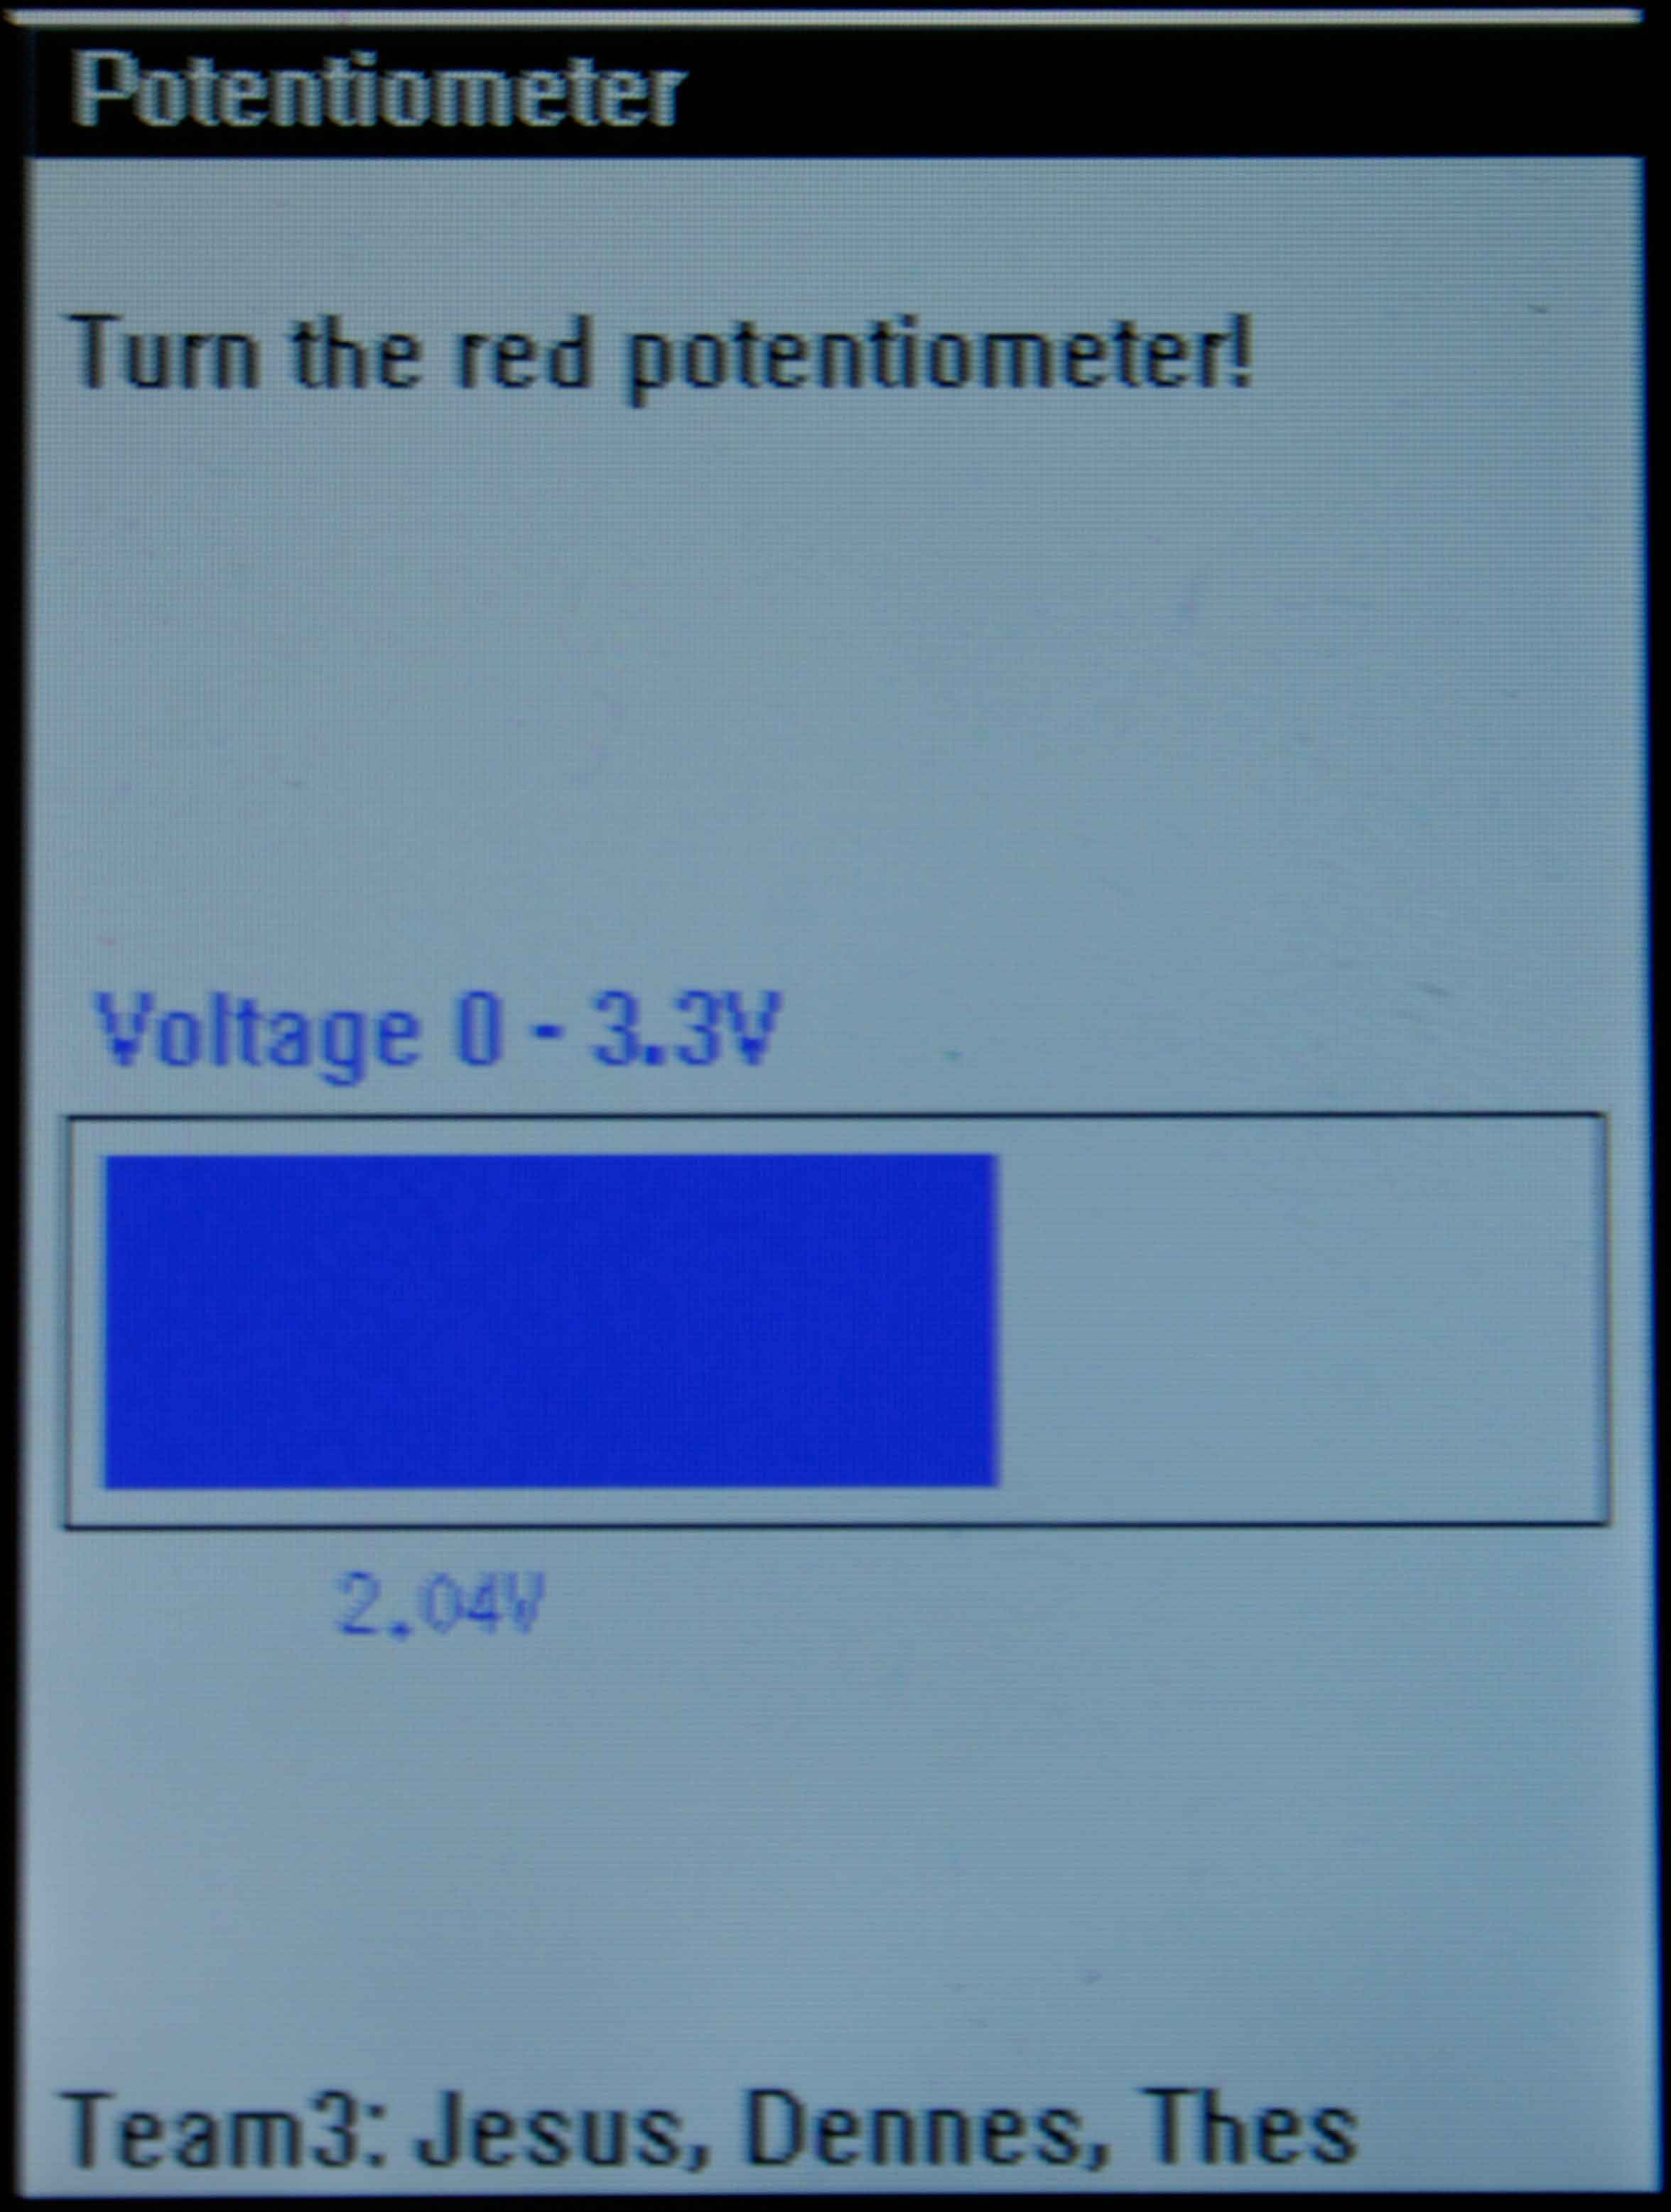
\includegraphics[width=0.4\textwidth]{potent.jpg}\\
   adc\_app.c : Show the values of all ADC channels & mess\_app.c : Show the value at the potentiometer above the LCD display. \\
\end{tabular}


\newpage

\end{document}
